% Application report section -- written by Huzaifa.
% Included from main.tex inside \section{Application and Calorie Module}.
% Numbers come from results/ood_thresholds.json, ood_val.csv, ood_test.csv and ood_probe.csv.
\subsection{Web Application Architecture and Interface}

The trained EfficientNet-B0 is served through a web application with two parts:
a Python backend that runs the model, and a browser frontend where the user
uploads a photo. Both run locally on a laptop; hosting was out of scope for this
deliverable. The backend lives in \texttt{app/backend/} and the frontend in
\texttt{app/frontend/}. A single command, \texttt{./run.sh}, starts both.

\subsubsection{Backend}
The backend is a FastAPI application (\texttt{app/backend/main.py}) with the
endpoints in Table~\ref{tab:endpoints}.

\begin{table}[H]
  \centering
  \small
  \begin{tabular}{|l|p{10.2cm}|}
    \hline
    \textbf{Endpoint} & \textbf{Purpose} \\ \hline
    \texttt{GET /health} & Status, number of classes, thresholds and whether the
      calorie module is available. \\ \hline
    \texttt{GET /dishes} & The 14 dish names. \\ \hline
    \texttt{POST /predict} & Takes an image (at most 10~MB) and an optional
      \texttt{portion} between 0.25 and 4. Returns the top 3 dishes with
      confidence, an \texttt{in\_scope} flag with a \texttt{reason} when the photo
      is rejected, and the calorie range. \\ \hline
    \texttt{GET /calories} & Calorie range for a chosen dish and portion, without
      running the model. Used after a user correction. \\ \hline
    \texttt{POST /feedback} & Stores the dish a user says the photo really shows
      (one of the 14 dishes, or \texttt{none}). \\ \hline
  \end{tabular}
  \caption{Backend endpoints.}
  \label{tab:endpoints}
\end{table}

\texttt{app/backend/model\_service.py} loads
\texttt{checkpoints/efficientnet\_best.pt} once, when the server starts, and keeps
the model in memory in evaluation mode. Each uploaded image is opened with Pillow,
rotated according to its EXIF orientation (phone photos often store rotation
there), converted to RGB, and passed through the same validation transform used
in training (\texttt{eval\_transforms()} in \texttt{src/dataset.py}: resize to
$224 \times 224$ and ImageNet mean and standard deviation). Reusing that function
means the application cannot drift away from the preprocessing the model was
evaluated with. The softmax output gives the top 3 classes, and the 1280-value
feature vector in front of the classifier is kept for the out-of-scope check
below. An unreadable file returns status 400, a file over 10~MB returns 413, and
a \texttt{portion} outside 0.25 to 4 returns 422.

\subsubsection{Out-of-scope check}
A classifier with 14 outputs must name one of them even for a photo that is not
one of the dishes. In our probe photos (below), a close-up photo of an arm
reached a top-1 confidence of 0.473, above the 0.45 confidence threshold chosen on
the validation set, so confidence alone would have accepted it as a dish. The application therefore rejects a photo if
either of two checks fails.
\begin{enumerate}
  \item \textbf{Confidence.} The top softmax probability must be at least
        $0.45$ (the threshold chosen on the validation set, described in the
        confidence threshold subsection below).
  \item \textbf{Similarity.} The cosine similarity between the photo's feature
        vector and the nearest of 14 dish centroids must be at least
        $0.4059$. The centroids are the mean feature vectors of the training
        images of each dish (\texttt{results/ood\_reference.npz}). The threshold
        was chosen on the validation set so that 88\% of correctly classified
        validation photos still pass; the script \texttt{src/ood\_analysis.py}
        computes it and writes \texttt{results/ood\_thresholds.json}.
\end{enumerate}
With both checks the model answers 75.7\% of the test images, with 88.2\%
accuracy on the answered ones (\texttt{results/ood\_test.csv}). A rejected photo
gets no calorie estimate: the interface says that the photo is not one of the
supported dishes and shows the 14 dishes.

We tested the rejection on 30 photos that are not dishes
(\texttt{results/ood\_probe.csv}): 26 random scenery and object photos from a free
photo site, and four photos we supplied (three portraits and the arm close-up).
29 of the 30 were rejected, all by the similarity check; the one that passed was a
photo of a desert dune, whose similarity (0.407) was barely above the threshold.
The set is small, informal and mostly scenery, so it shows that the check works
on common cases, not that it catches every non-dish photo. Tightening the
threshold would reject more non-dish photos but also more real dishes, because
the similarity threshold is a trade-off.

\subsubsection{User feedback}
Under every answer the interface asks ``Is this correct?''. \emph{Yes} confirms the
answer. \emph{No} opens a picker that lists the model's other guesses first, then
all 14 dishes and a ``None of these'' option; choosing a dish immediately shows
that dish with its calories, and the user can change the answer again. Photos
rejected as out of scope can be corrected in the same way if the dish was
wrongly rejected.

Each answer is saved by the backend as one line in
\texttt{feedback/corrections.jsonl} together with the photo. A record holds an
identifier, a UTC timestamp, the image file and its SHA-256 hash, the predicted
label, confidence and top three guesses, the in-scope flag and reason, the
corrected label and whether the model was right. The backend runs the model
itself on the posted photo, so the stored prediction cannot be edited by the
client. Photos are re-saved as JPEG, which drops EXIF data such as location, and
the \texttt{feedback/} folder is excluded from Git because it holds user photos.
The records can be used later to evaluate or retrain the model.

\subsubsection{Tests}
Three test files cover the application. \texttt{tests/test\_api.py} (six tests)
checks the health and dish endpoints, the shape of a prediction, and that a
non-image file, a bad portion and a flat colour image are handled correctly.
\texttt{tests/test\_ood.py} (six tests) checks the rejection logic.
\texttt{tests/test\_feedback.py} (five tests) checks the calories and feedback
endpoints; these write to a temporary folder. The tests that load the model are
skipped when the weights file is absent.

\subsubsection{Frontend}
The frontend is a React application built with Vite
(\texttt{app/frontend/src/}). During development it forwards requests under
\texttt{/api} to the backend on port 8000. Its main parts are:
\begin{itemize}
  \item \textbf{Upload and camera:} drag and drop, a file picker, or a photo taken
        with the device camera, with a clear message when camera permission is
        blocked.
  \item \textbf{Result card:} the dish name, the confidence, and two tiles with
        the typical energy and the likely range, followed by the serving
        description and an expandable list of the sources behind the numbers.
  \item \textbf{Portion picker:} Small ($0.75\times$), Regular ($1\times$), Large
        ($1.5\times$) and Double ($2\times$). Choosing one asks the backend for
        the new calorie values, so the numbers always come from the server.
  \item \textbf{Top guesses:} the three most likely dishes with their
        confidences, drawn as a menu with dotted leaders.
  \item \textbf{Feedback and picker:} the ``Is this correct?'' control and the
        out-of-scope screen described above.
  \item \textbf{Session history:} the last six photos and their results, kept in
        memory only.
\end{itemize}
The visual design follows an organic editorial style: a cream and deep green
palette with terracotta accents, a high-contrast serif for headlines, a large
food photograph in the opening section, and a calorie card that overlaps the
photo. There is a light and a dark theme. The interface uses short transitions
(scroll reveals, a slight parallax on the opening photo, counting numbers and
growing bars), which are switched off when the user's system asks for reduced
motion. The opening photo is by Shreyak Singh from Unsplash.

\subsubsection{Interface examples}
Figure~\ref{fig:app-landing} shows the opening screen and Figure~\ref{fig:app-result}
a confident prediction for a chicken biryani photo from the test set.
Figure~\ref{fig:app-feedback} shows the picker that opens when the user presses
\emph{No}. Figure~\ref{fig:app-oos} shows a photo that is not a dish, here a flag,
which the application rejects without a calorie estimate and with the dish list
instead.

\begin{figure}[H]
  \centering
  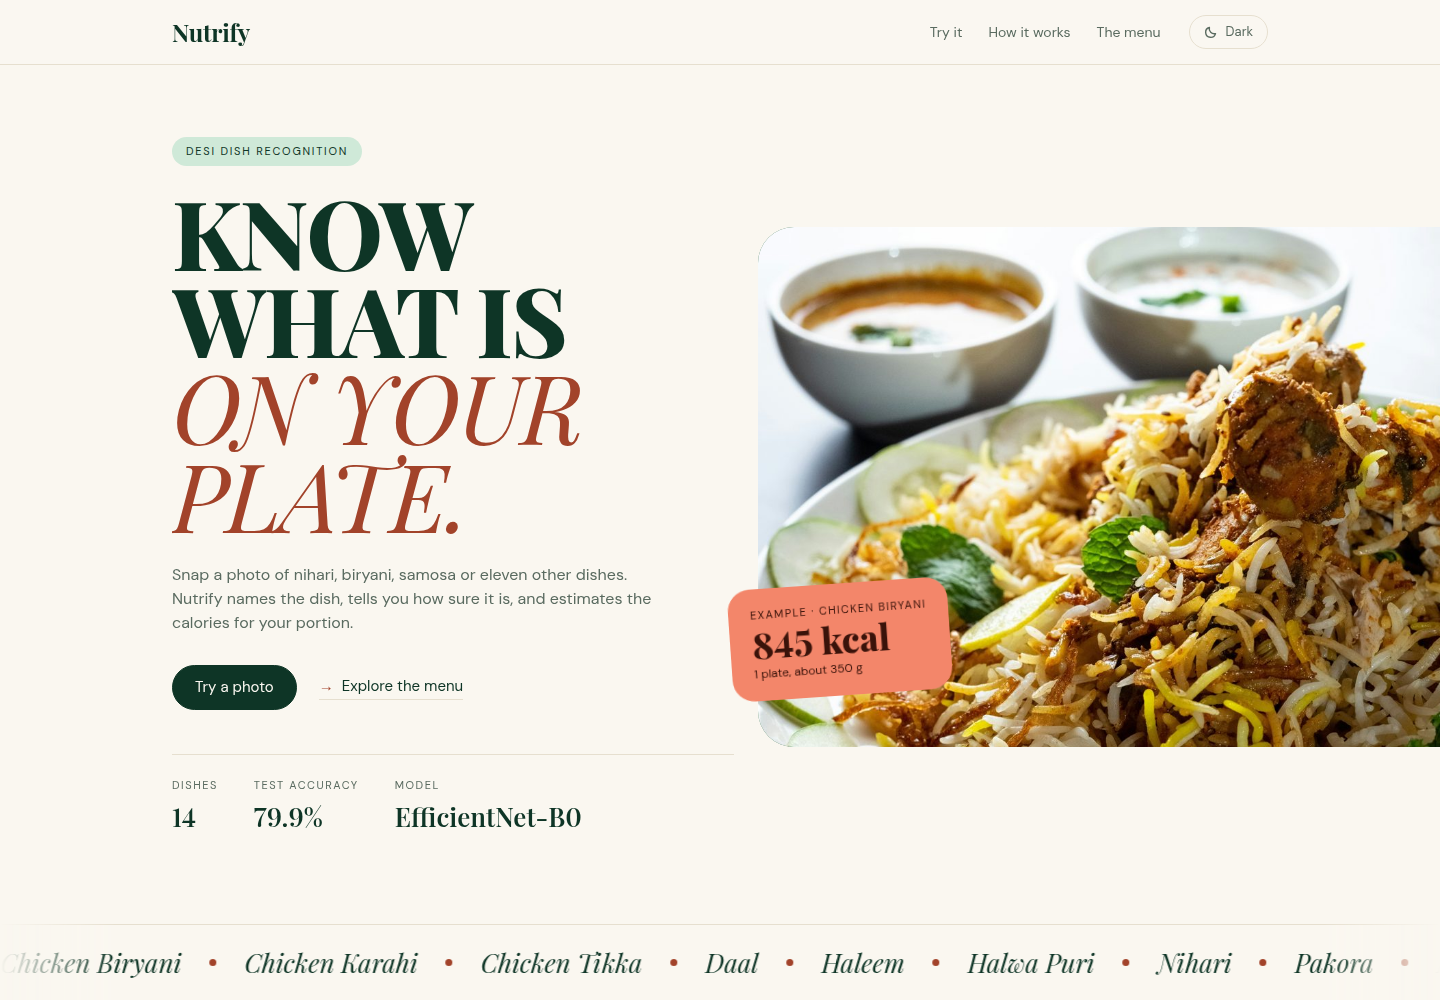
\includegraphics[width=0.95\textwidth,height=0.5\textheight,keepaspectratio]{app_landing.png}
  \caption{Opening screen of the application (light theme).}
  \label{fig:app-landing}
\end{figure}

\begin{figure}[H]
  \centering
  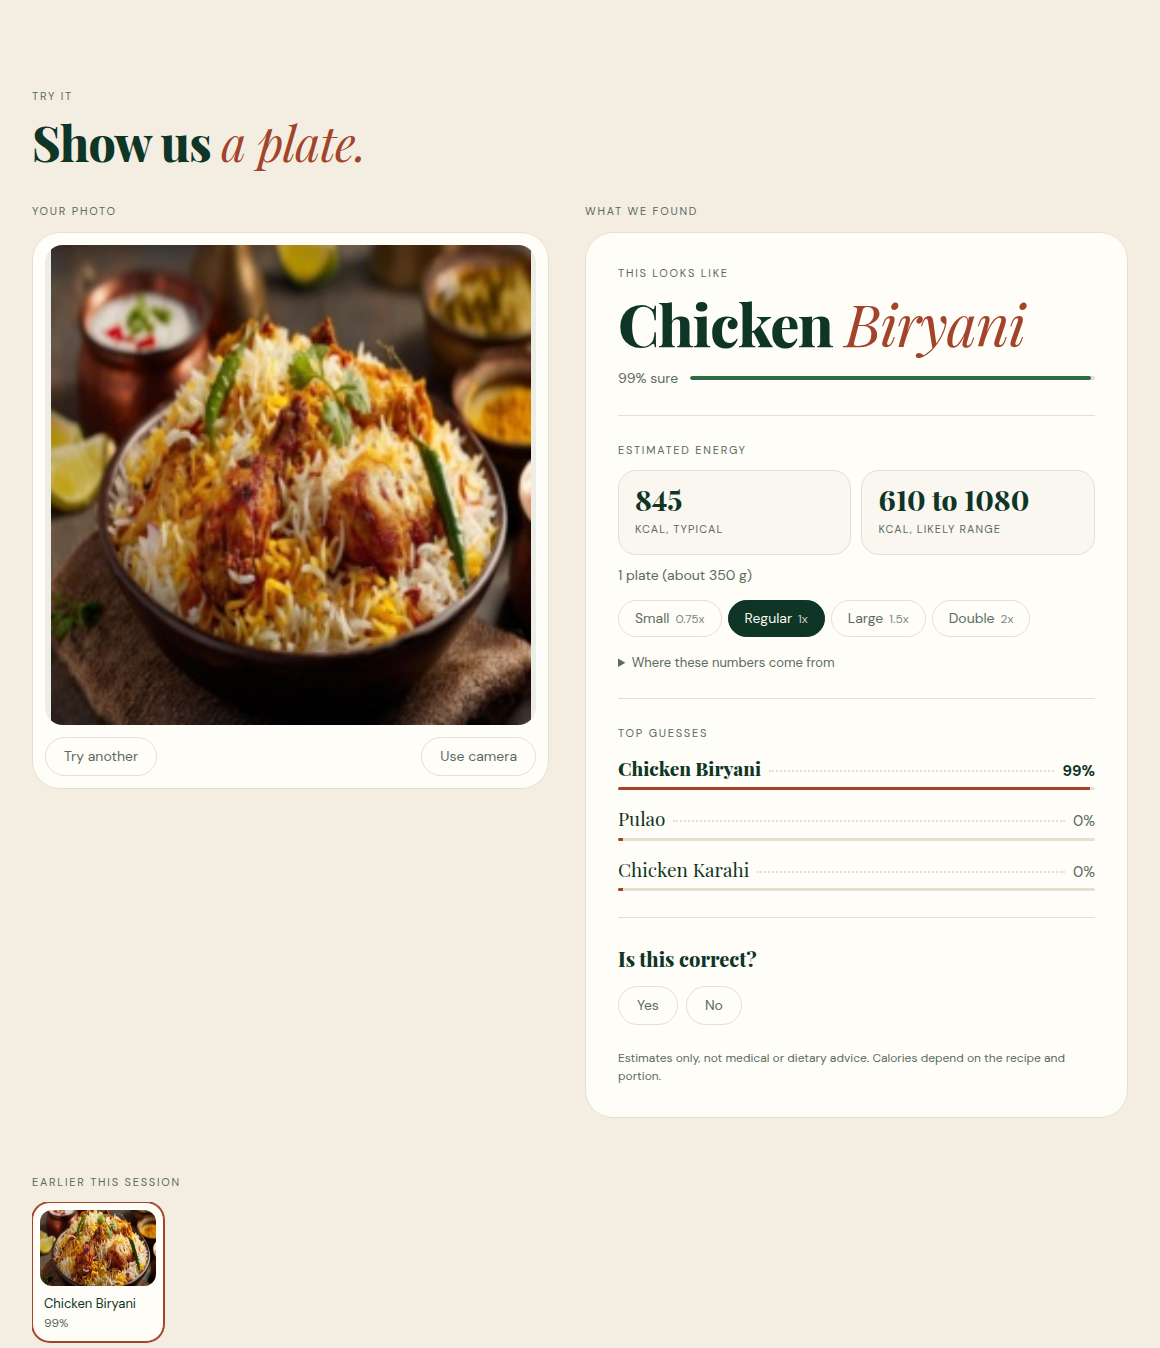
\includegraphics[width=0.8\textwidth,height=0.55\textheight,keepaspectratio]{app_screenshot.png}
  \caption{Confident prediction: dish, confidence, calorie tiles, portion pills,
  top three guesses, the feedback question and session history.}
  \label{fig:app-result}
\end{figure}

\begin{figure}[H]
  \centering
  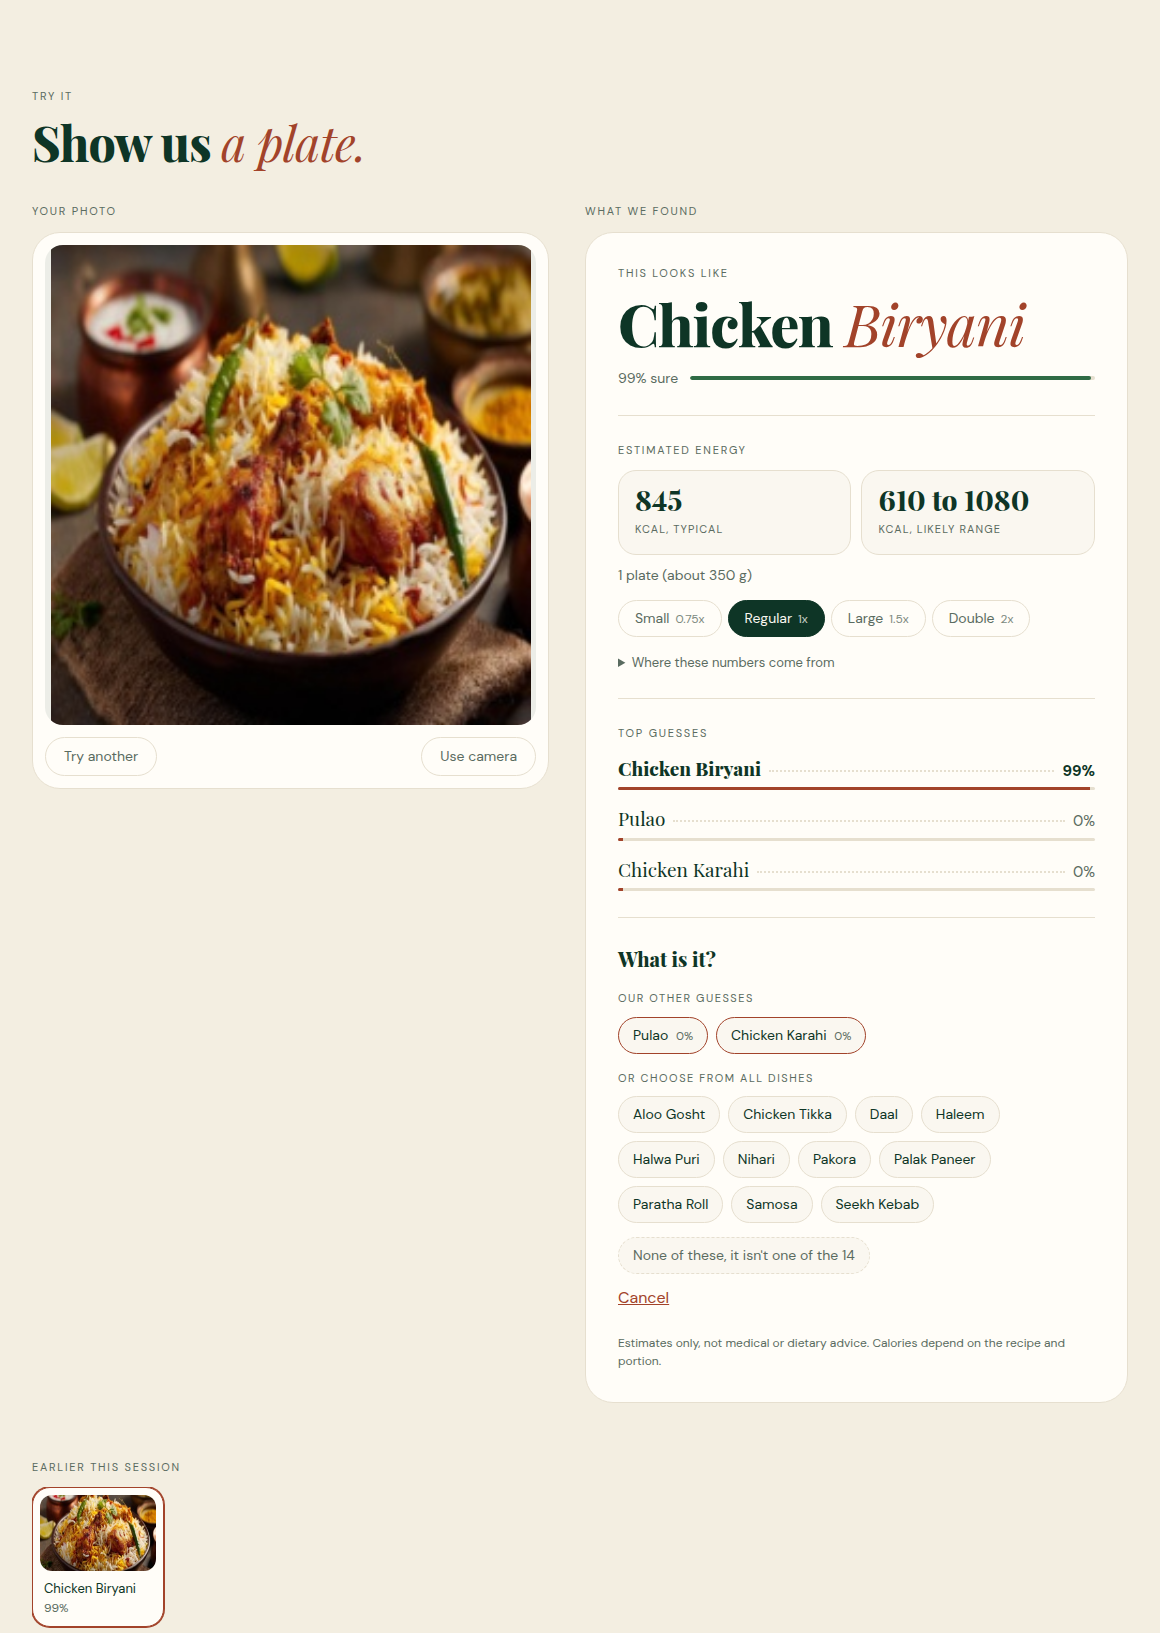
\includegraphics[width=0.8\textwidth,height=0.55\textheight,keepaspectratio]{app_feedback.png}
  \caption{After pressing \emph{No}: the user picks the right dish from the model's
  other guesses or from all 14 dishes, or chooses ``None of these''.}
  \label{fig:app-feedback}
\end{figure}

\begin{figure}[H]
  \centering
  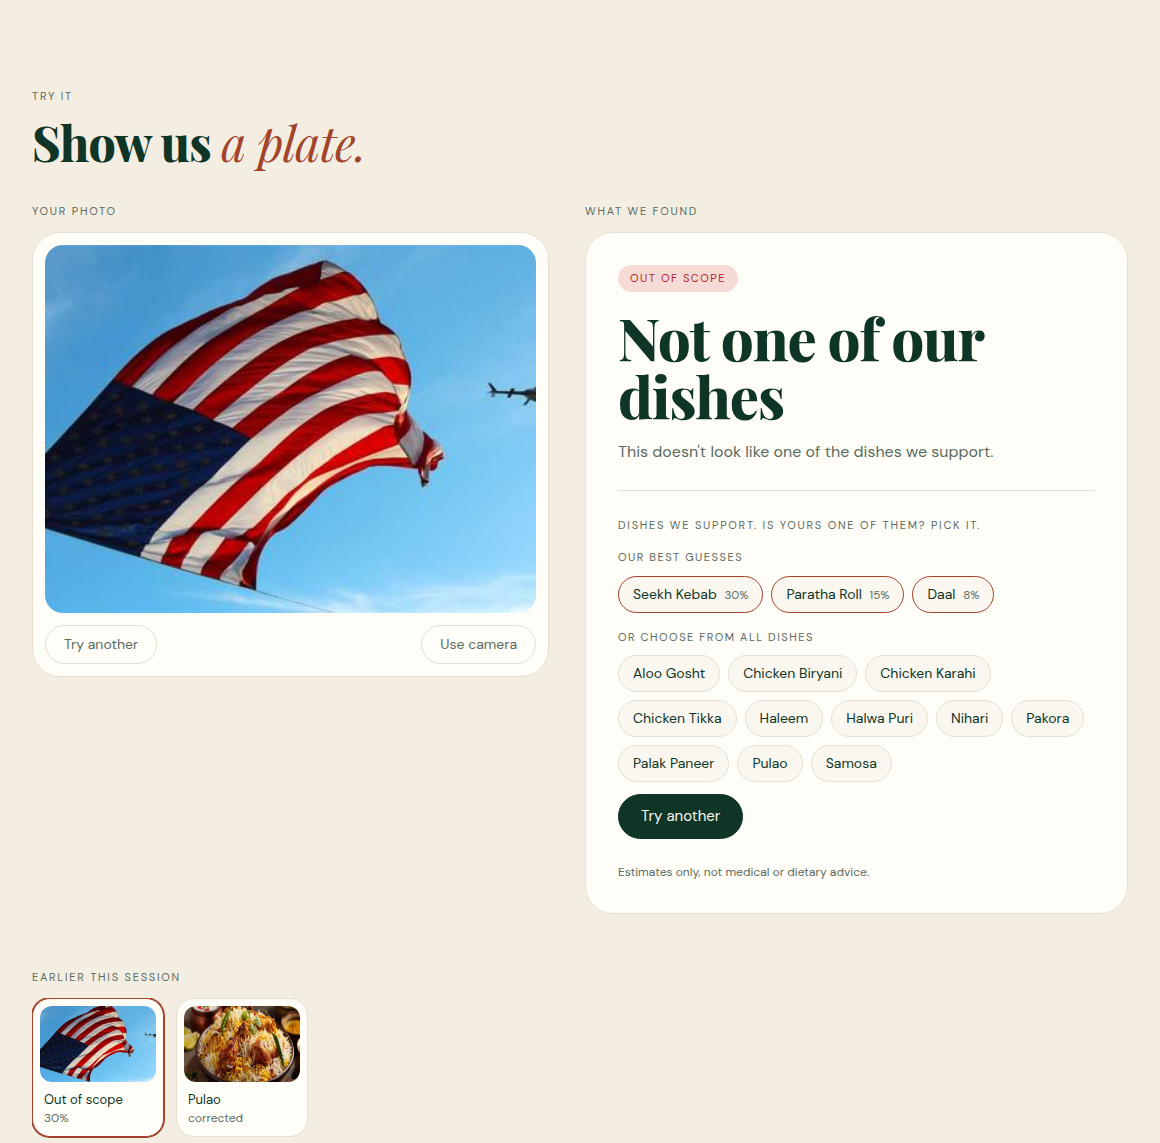
\includegraphics[width=0.8\textwidth,height=0.55\textheight,keepaspectratio]{app_out_of_scope.png}
  \caption{A photo that is not a dish is rejected: no calories, the supported
  dishes, and the option to pick the right dish if the rejection was wrong.}
  \label{fig:app-oos}
\end{figure}

The application does not detect the portion size from the photo. The user
chooses it, and the calorie numbers are estimates from recipes and food
composition tables (see the calorie and threshold limitations below).
